\section{Programas de estudio}
En términos generales, se puede definir un programa de estudios como una herramienta educativa que regula y ordena el proceso de enseñanza-aprendizaje a desarrollar en una unidad de aprendizaje determinada, orientando las actividades que profesor y alumno han de llevar a cabo para el logro de los objetivos planteados en dicha unidad, en relación con los objetivos del plan de estudios, de tal manera que el egresado concluya su carrera con el perfil deseado. En pocas palabras, es un esquema organizado de los contenidos situados dentro de una determinada unidad de aprendizaje\citep{lalor_ensuring_2017}.

El termino \enquote{unidad de aprendizaje} sustituye al de \enquote{asignatura} o \enquote{materia} que evocan los tradicionales cursos unidisciplinarios, generalmente teóricos y sobrecargados de información. Un programa resume las características de la unidad de aprendizaje, su contenido mínimo obligatorio, y sus objetivos, principalmente.

En la primera etapa de diseño curricular, se requiere la elaboración de la propuesta de los programas para su aprobación de parte de las autoridades con la colaboración de las academias y, de ser necesario, con la asesoría de externos de la unidad académica.

\subsection{Proceso de diseño curricular} \label{procesoCurricular}
Para aquellas personas ajenas al entorno educativo, en específico aquellas que no forman parte del proceso de diseño curricular puede ser un tanto complejo el proceso de creación y revisión de material curricular en las instituciones. En la actualidad, un formulario de creación o revisión de competencias, cursos, y programas debe pasar por una serie de evaluadores (figura \ref{flujo_autoridades}) que son los encargados de revisar y verificar que los datos sean válidos.
\begin{figure}[H]
\centering
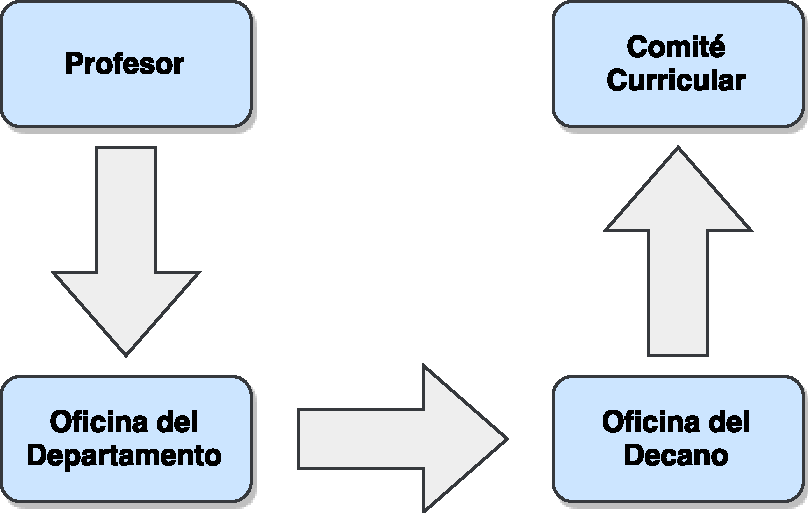
\includegraphics[scale=0.5]{Capitulos/MarcoTeorico/Imagenes/flujo_autoridades}
\caption{Flujo de creación y revisión de propuestas.}
  \label{flujo_autoridades}
\end{figure}

Hoy día el estado de California cuenta con un patrón de definición de cursos y programas donde la misma sirve como guía para el desarrollo de propuestas para material académico de las universidades. Dicho estándar además contiene una taxonomía de programas e indica cuál es el flujo para la revisión de las propuestas, donde todo es establecido en el PCAH\footnote{de sus siglas en inglés, Program and Course Approval Handbook, que significa en español manual de aprobación de cursos y programas.}\citep{brice_w_harris_program_2013}.

El flujo inicia con el profesor o encargado del curso o programa, una vez completado pasa por la mesa de recepción donde se verifica que cumpla con el estándar estatal para luego pasar por la oficina departamental y la oficina del decano para su revisión de contenido. Una vez revisado y con el visto bueno de ambas oficinas pasa por una última revisión por parte de la oficina curricular para ser registrada en los sistemas de gestión curricular (figura \ref{course_creation_flow}).

Es un proceso que se hace con formularios en papel donde el profesor o encargado del curso o programa tiene que completar los campos requeridos para que el estado de California cuente al curso como válido. Dicho proceso tiene varias deficiencias:
\begin{itemize}
	\item La creación o revisión puede tomar meses debido a los formularios que son completados a mano y requieren de revisión de varias oficinas.
	\item Es un flujo de una sola dirección, eso quiere decir que si es que una de las oficinas rechaza el formulario debe volver a iniciar el flujo.
	\item Se puede producir cuellos de botella en los diferentes puntos de revisión.
\end{itemize}

Una vez ya registrado en los sistemas de gestión curricular es accesible de manera pública para el uso de las universidades del estado de California. De esta manera, si una institución académica posee un sistema de gestión de evaluaciones y quiere incluir los cursos o programas válidos para el estado tiene que ingresar los nuevos datos del sistema de gestión curricular uno a uno como se puede apreciar en la figura \ref{after_creation}.

\begin{figure}
\centering
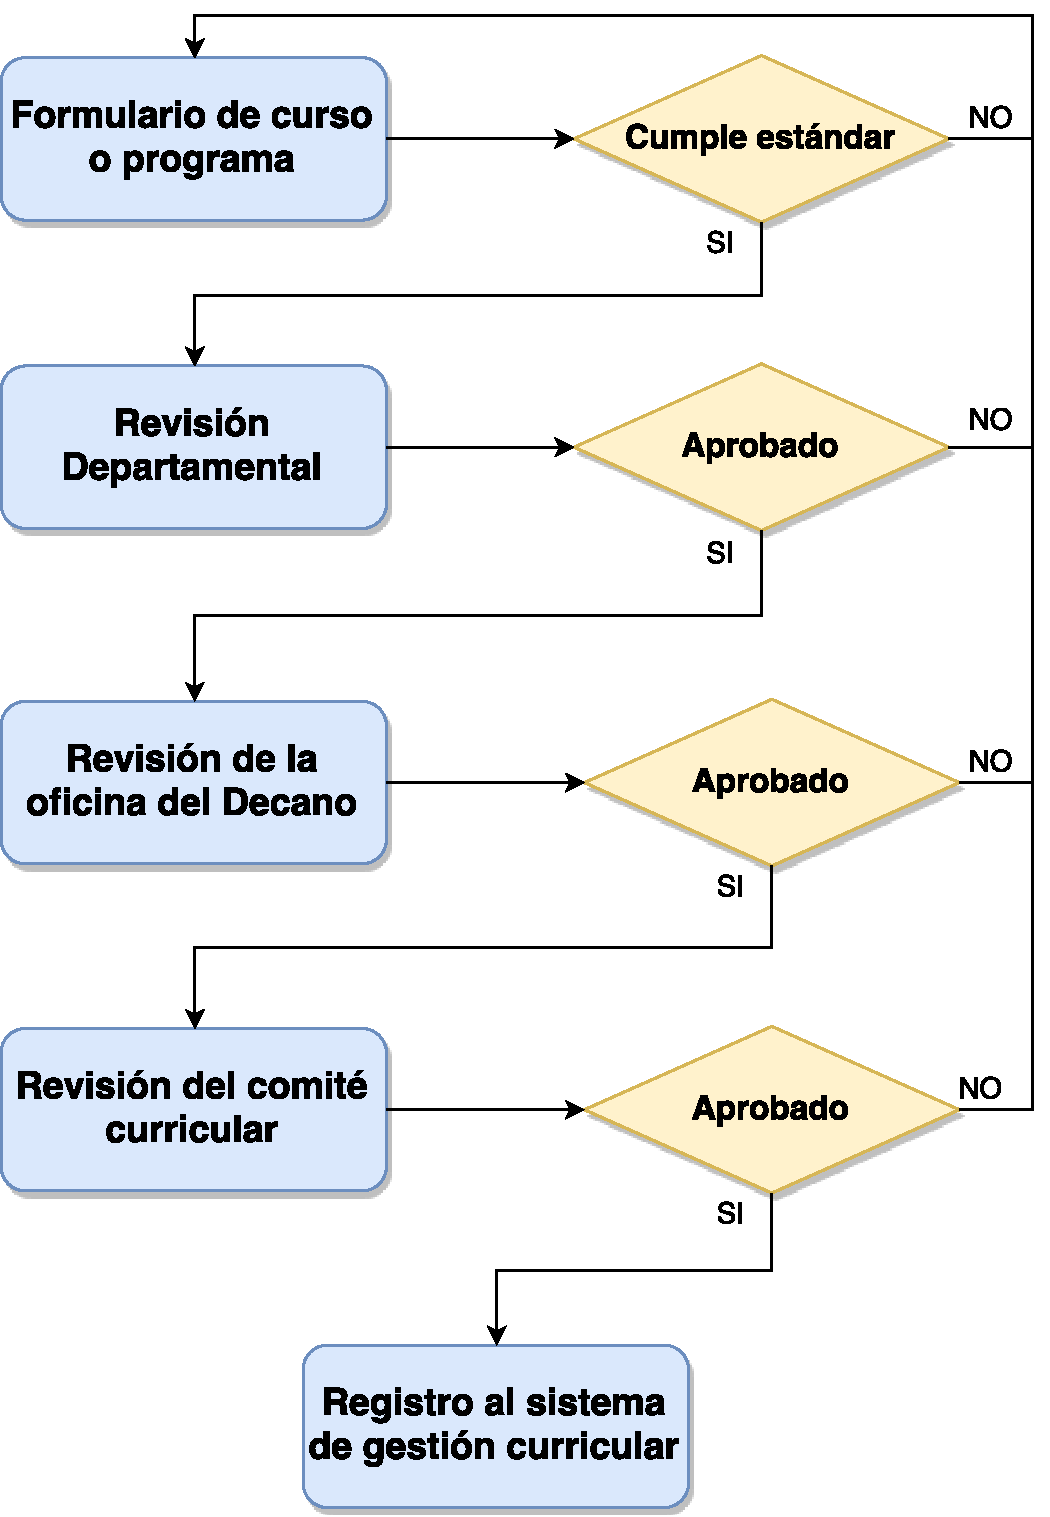
\includegraphics[scale=0.5]{Capitulos/MarcoTeorico/Imagenes/course_creation_flow}
\caption{Flujo actual de diseño de cursos, programas y competencias.}
  \label{course_creation_flow}
\end{figure}

\begin{figure}
\centering
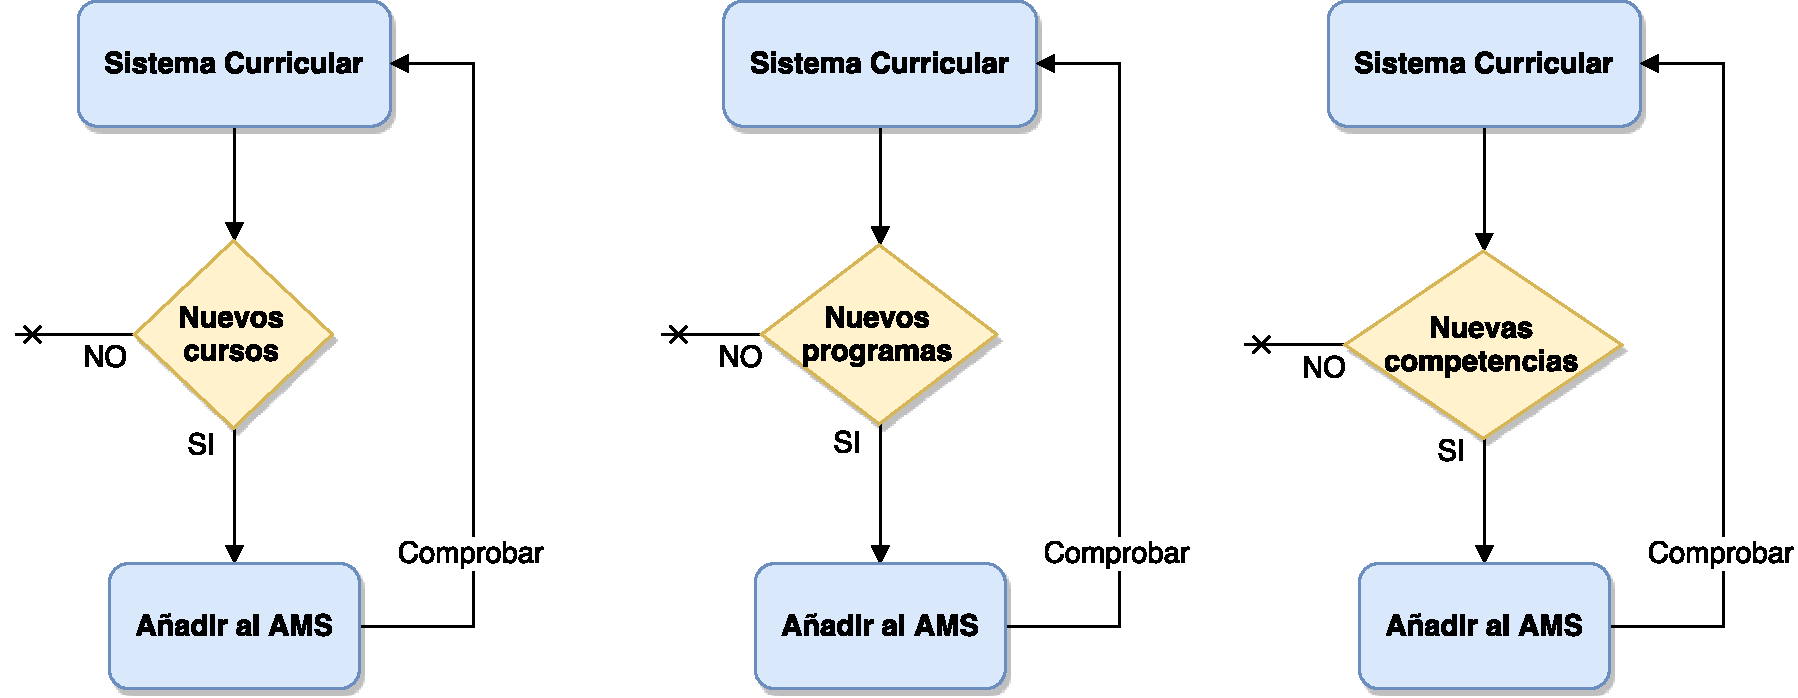
\includegraphics[width=125mm,scale=1]{Capitulos/MarcoTeorico/Imagenes/after_creation}
\caption{Esquema de tipos de computación en la nube.}
  \label{after_creation}
\end{figure}